\documentclass[12pt,english]{article}
\usepackage[utf8]{inputenc}
\usepackage{tgpagella} % Palatino text only
\usepackage{mathpazo}  % Palatino math & text
\usepackage[left=1.5in,right=1.5in,top=1.5in,bottom=1.5in]{geometry}
% \linespread{1.5}
% \usepackage[super,comma,sort]{natbib}
\usepackage[round,sort&compress]{natbib}
\usepackage{url} % [hyphens]
\usepackage[hyperpageref]{backref} % back references biblio. Needs latexmk at compilation.
\usepackage[pagebackref]{hyperref}
% \usepackage{multibib} % incompatible with backref
\hypersetup{
  colorlinks=true, % breaklinks=true,
  urlcolor=purple,    % color of external links
  linkcolor=blue,  % color of toc, list of figs etc.
  citecolor=violet,   % color of links to bibliography
}
\usepackage{bm}
\usepackage{indentfirst}
\usepackage{tocbibind}
\setcitestyle{aysep={}} 
\usepackage{amsmath}
\usepackage{amssymb}
\usepackage{eurosym}
\usepackage{amsfonts}
\usepackage{enumerate}
\usepackage{babel}
\usepackage{caption}
\usepackage{supertabular}
\usepackage{tabularx}
\usepackage{float}
\usepackage{dsfont}
\usepackage{fancyvrb}
\usepackage{verbatim}
\usepackage{enumitem}
\usepackage{setspace}
\usepackage{comment}
\usepackage{subcaption}
\usepackage{graphicx}
\usepackage{tikz}
\usepackage{gensymb}
\usepackage{textcomp}

\usepackage{tabulary}
\usepackage{tabularx}
\usepackage{booktabs}
\usepackage{fullpage}
\usepackage{morefloats}
\usepackage{makecell}
\usepackage{lscape}
\usepackage{pdflscape}
\usepackage{longtable}
\usepackage{rotating}
\usepackage{xcolor}% header
\usepackage{titlesec} % To change size of Bibliography heading
\usepackage{fancyhdr}

% Header on every page except frontpage (handled by tikz)
% \pagestyle{fancy}% header
% \renewcommand{\headrulewidth}{0pt} % removes horizontal line from header
% \setlength{\headheight}{62pt} % adjust the nb of pt here and below if there is a warning
% \addtolength{\topmargin}{-62pt}
% \fancyhead[R]{} % removes section title from header
% \fancyhead[L]{} % removes section title from header
% \chead{\href{http://global-redistribution-advocates.org}{
\includegraphics[height=1cm]{../figures/policies/logo_full_white_bg}}\\ \quad }

\usepackage{tocloft}
\usepackage{titletoc}
\usepackage{csquotes}
\usepackage{tcolorbox}
\usepackage[export]{adjustbox}
\usepackage[anythingbreaks]{breakurl} % for links
\usepackage{multicol}
\newsavebox\ltmcbox % For net gain table over two columns
%\usepackage[nomarkers,figuresonly]{endfloat} % Figures at the end
%\usepackage[section,below]{placeins} % Floats placed in the section they appear in.
\renewcommand{\floatpagefraction}{.9}

\title{The Global Climate Assembly -- Policy Brief
} 

\author{\textcolor{white}{Adrien Fabre\footnote{\textcolor{black}{The author is Adrien Fabre, CNRS researcher in economics at CIRED. E-mail: adrien.fabre@cnrs.fr.}}}
%\footnote{CNRS researcher in economics at CIRED. E-mail: adrien.fabre@cnrs.fr.}
} 
% \author{Global Redistribution Advocates\footnote{The author is Adrien Fabre, CNRS researcher in economics at CIRED. E-mail: adrien.fabre@cnrs.fr.}} 

\date{\today{} -- \href{https://github.com/bixiou/global_tax_attitudes/raw/main/paper/policy_brief_assembly.pdf}{Link to most recent version}} 

\begin{document}

\maketitle
\tikz [remember picture, overlay] %
\node [shift={(5.5cm,-1.5cm)}] at (current page.north west) % north west
[anchor=north west] % north west
{\href{http://global-redistribution-advocates.org}{
\includegraphics[height=1.3cm]{../figures/policies/logo_full_white_bg}}};

% \begin{center}
% {\textbf{\href{https://github.com/bixiou/global_tax_attitudes/raw/main/paper/policy_brief_GCP.pdf}{Link to most recent version}}}
% \end{center}

\begin{figure}[h!] 
    \caption{Support for the Global Climate Assembly around the World (in percent).}\label{fig:support}
    \makebox[\textwidth][c]{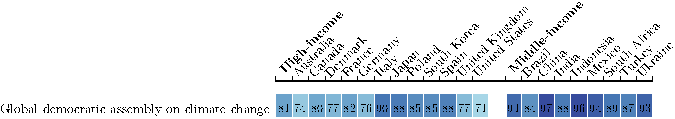
\includegraphics[width=1.2\textwidth]{../figures/OECD/Heatplot_global_tax_attitudes_only_democracy_share.pdf}} 
\end{figure}

\section{Summary}\label{sec:intro}
\citet{fabre_international_2023} survey attitudes toward global policies in 20 among the largest countries and find near consensus for ``a global democratic assembly whose role would be to draft international treaties against climate change.'' In this Global Climate Assembly (GCA), ``Each adult across the world would have one vote to elect members of the assembly.'' 

In this policy brief, we defend a GCA with proportional representation: For the first time, a global election would be held, with citizens of participating countries making the same choice between different lists in a unique constituency. 12 lists would be eligible, those obtaining the largest endorsement in a pre-election petition, provided that they obtain more than 1 million signatures. No restriction would be placed on the composition of the lists, except that one person could only appear in one list. 

The GCA would propose to the UNFCCC an international treaty on climate change and would represent the world citizens in the international climate negotiations. %In the last months of its five-year mandate, reflecting on its experience, the GCA would deliberate on global governance and propose a governance framework to address climate change.

\section{Support}\label{sec:support}

% Surveys
Before \citet{fabre_international_2023}, who found near consensus in favor of the GCA in representative samples of 20 countries (see Figure \ref{fig:support}), several surveys have already shown widespread support for global democratic institutions. In surveys in Brazil, Germany, Japan, the UK and the U.S., \citet{ghassim_who_2020} finds 55 to 74\% of support for ``a global democracy including both a global government and a global parliament, directly elected by the world population, to recommend and implement policies on global issues''. % (for example, international peace, world poverty, and climate change)''
Using an experiment, he also finds that, in countries where the government stems from a coalition, voting shares would shift by 8 (Brazil) to 12 p.p. (Germany) from parties who are said to oppose global democracy to parties that supposedly support it. For example, when Germans respondents were told that (only) the Greens and the Left support global democracy, these parties gained respectively 9 and 3 p.p. in vote intentions while the SPD and the CDU-CSU each lost 6 p.p.  
\citet{ghassim_who_2020} also document survey results which show strong majorities support in each of 18 countries for the direct election of one's country's UN representative. % same as unpa_survey_2005 % GlobeScan 2005; also: half/half (majorities or not depend on the country) for “Global Parliament, where votes are based on country population sizes, and the global parliament is able to make binding policies” (Synovate 2007); also: (GlobeScan 22, not from Ghassim) in 31 countries: 77% agree that “Rich countries must pay for poorer countries do deal with the effects of CC” 
Similarly, in each of 10 countries, there are clear majorities in favor of ``a new supranational entity [taking] enforceable global decisions in order to solve global risks'' \citep{global_challenges_foundation_attitudes_2018}. Actually, already in 1946, 54\% of Americans agreed (and 24\% disagreed) that ``the UN should be strengthened to make it a world government with the power to control the armed forces of all nations'' \citep{gallup_seventy_1946}. 
In surveys in Argentina, China, India, Russia, Spain, and the U.S., \citet{ghassim_public_2022} find majority support for UN reforms that would make United Nations' decisions binding, give veto powers at the Security Council to a few other major countries, or complement the highest body of the UN with a chamber of directly elected representatives. 

% Relatedly, \citet{meilland_international_2023} find that Americans and French people prefer an international settlement of climate justice even if it empedes on sovereignty. In a 2013 survey in China, Germany and the U.S., \citet{schleich_citizens_2016} show that more than three quarter of people think that international climate agreements reached so far are not successful and that future agreements are important. % 73\% of people find important future international climate agreements, while less than 26\% think that international reached so far are successful. 
% In Finland, \citet{sivonen_attitudes_2022} finds that a carbon tax receives higher support if enacted at the global level (54\%) rather than at the national level (40\%).

% These specific questions are in line with the answers to more general questions. In each of 36 countries, \citet{issp_international_2010} find near consensus that ``for environmental problems, there should be international agreements that [their country] and other countries should be made to follow'' (overall, 82\% agree and 4\% disagree). % No question like this in the next Envi wave in 2022
% In each of 29 countries, \citet{issp_international_2019} uncover near consensus that ``Present economic differences between rich and poor countries are too large'' (overall, 78\% agree and 5\% disagree). 

\section{Movements for a global constituency}
% Existing campaigns
Since \citet{kant_zum_1795}, for whom world federalism was the necessary condition for perpetual peace, many have argued that we need stronger and more democratic global institutions, competent to address global challenges like extreme poverty, climate change, wars, pandemics, or financial stability. 
Before World War II, feminist and pacifist \citet{maverick_lloyd_chaos_1937} founded the \textit{Campaign for World Government}, defending direct representation at the global scale. 
\citet{einstein_general_1947} called for the subordination of the UN Security Council to the General Assembly and the direct election of UN delegates. 

Since 2007, individuals and institutions from more than 150 countries have endorsed the appeal for a United Nations Parliamentary Assembly (UNPA), including 1,800 member of parliament, heads of state, as well the European Parliament, the Pan-African Parliament, and the Latin-American Parliament. The UNPA calls for a gradual implementation of a democratic assembly, starting with a consultative assembly composed of members of national parliaments, allowing for the direct election of its members in voluntary countries, and evolving toward a world parliament able to adopt binding regulations once all members are directly elected \citep{leinen_world_2018}. % READ Ch 13, 21, 22, 26
Besides the UNPA, various scholars have proposed different models of global democracy, ranging from deliberative spaces to a world federation \citep{archibugi_global_2011}. % TODO READ and expand, also read marchetti_global_2008
%Using surveys covering 86\% of global population, \citet{hale_could_2019} find that the world as a whole is less polarized that some countries and argue against the fear people's views would be too diverse for a functioning global democracy. 
While the most radical proposals are still out of sight, an assembly of random citizens representative of the world population has already been convened. It has produced a joint statement at the COP26 \citep{global_assembly_report_2022}, and a similar \textit{World Citizens' Assembly} should soon follow. 
% Stanford dico (kuyper_global_2016)? 

\section{Rationale for a GCA}

% rationale
The GCA would entail the first intercontinental election with universal suffrage. As such, the GCA's experimental status should be assumed. The GCA would not have any enforcement capacity, to avoid the risks inherent to a first-of-its-kind experiment. 
The GCA should be understood as a prototype of a permanent global assembly, and similar attempts can be iterated until we find a suitable institutional arrangement. 

Beyond the institutional lessons it would teach, the GCA's proposals on global climate policy could greatly enhance international climate negotiations. Indeed, the GCA's deliberations might offer a forum where national interests could be overcome. Actually, the electoral campaign itself could reveal wide agreement in favor of some specific form of climate action. For instance, \citet{fabre_international_2023} reveal majority support in the 20 countries surveyed for a \href{https://github.com/bixiou/global_tax_attitudes/raw/main/paper/policy_brief_GCS.pdf}{Global Climate Plan}, suggesting that the values of world citizens are more aligned than the positions of governments. The electoral campaign could also yield intrinsic benefits, such as raising awareness on climate justice or facilitating the emergence of global media entertaining a global public debate. 

We support the UNPA campaign, and see the UNPA as complement (not substitute) to the GCA. While the former attempts to reform the UN, the latter tries to build another space for global deliberation. The GCA might prove more achievable than the UNPA, as it can be established by a subset of all countries independently from the UN dynamics. Furthermore, the GCA uses a different approach that could garner more support. First, it is more modest, as it only aims at a one-off consultative assembly, not a permanent one progressively endowed with binding power. Second, by focusing on climate-related issues, it could mobilize a wider base of activists than the UNPA, which mostly appeal to world federalists.  Third, by representing citizens based on their values rather than their country, the GCA goes beyond the defense of (conflicting) national interests. Indeed, by relying global lists of candidates, the GCA transcends the international approach and grants every world citizen an equal representation. On the contrary, as the UNPA seeks to represent each country, with at least two delegates per country --- including at least one from the opposition party \citep{leinen_world_2018}, it overrepresents citizens of small countries and risks alienating large countries. 

We also support initiatives such as the \href{https://globalassembly.org/}{Global Assembly} that gathers randomly selected citizens to deliberate on a given topic. We welcome these other experiments as they can also provide potential models of democratic institutions at the global scale. The great advantage of the Global Assembly is that it can be conducted by NGOs without needing the agreement of governments. Compared to random selection, one big advantage of the GCA lies in the electoral campaign, which would bring the public debate to the global level and spur global thinking.%, spur global conversation and foster global mobilization.


\section{Details of the GCA}\label{sec:details}

Although we are very open to the specific form that the GCA could take, we sketch below a possible arrangement as a proof-of-concept and a basis for discussion. 

The GCA would be established by an alliance of countries covering at least half of the world's adult population.\footnote{37\% of the world population live in an authoritarian regime according to the Democracy Index by \citet{eiu_democracy_2022}.} 
Our preferred option to encourage the participation of all countries is simply that only participating countries would be represented at the GCA. Alternatively,  governments refusing to organize the election could be allowed to choose delegates but would be penalized by receiving only half of the seats corresponding to their population; or, in countries refusing the election, we could randomly draw citizens and ask them to vote at the global election. 

The pre-election would last one year, during which lists would be deposited and endorsements gathered. For a list to be registered, it would need to contain as many members as there are seats (e.g., 400); each member would have a rank and could not be part of an already registered list. Crucially, no restriction would be placed on the composition of the lists: for instance, the members from a list could all come from the same country. % Campaign finance

At the end of the pre-election period, each list gathering more than one million endorsements would be screened. The authenticity of the endorsements would be checked by contacting a random sample of signatories. The pre-election expenses would be scrutinized, and any list which would have benefited more than \$20 million of spending would be disqualified. The remaining lists would be ordered by number of endorsements,\footnote{At this stage, endorsements of citizens who already endorsed a higher-ranked list would be canceled so that each person can only endorse one running list.
% and prevent manipulation
} and the most supported (up to a limit of 12 lists) would be qualified to run at the election. Each running list would be granted \$50 million to cover its pre-election and campaign expenses. No extra funding would be allowed, on penalty of disqualification.

The election would occur six months after the qualified lists are known. During the campaign, debates between members of the competing lists would be organized in different languages. Each list would prepare a flyer with its platform. The IPCC would study the flyers, assess the outcomes of the respective proposals and flag any inaccuracies. The IPCC would also prepare its own flyer to summarize its report. An outlet containing all flyers would be distributed to each voter before the election. The ballots would be secret. 

% Sessions
The seats would be allocated proportionally to the voting shares (rounding would preferably use the Hare quota in the largest-remainder method). Ideally, the GCA would be located in a country that does not already host a major international organization, such as Ghana or India. The delegates would be appointed for a unique mandate of five years. Each delegate will receive a salary and the budget to employ an assistant. 

The debates and votes of the GCA and its committees should be public. The GCA would further specify its internal rules within the first six months of its mandate. The rules should specify the methods of agenda setting, the amendment and voting procedures, as well as the selection method for appointing representatives to other institutions (like the UNFCCC). The delegates would elect a President during the first sessions using the \href{https://en.wikipedia.org/wiki/Combined_approval_voting}{combined approval voting} method. To propose internal rules, the President would form a committee of delegates, with at least one delegate from each list that obtained more than 5\% of the seats, their mandate would expire after six months. The internal rules should be adopted by the plenary assembly (with a positive score in a combined approval vote). If, after six months, no internal rules have been adopted, the Secretary-General of the UN would appoint a qualified person to choose these rules. 

The GCA would present the advancement of its work at the UNFCCC's COP every year. The role of the GCA would be to propose an international treaty on climate change within the first four year of its mandate. In the last six months of its five-year mandate, reflecting on its experience, the GCA would deliberate on global governance and propose a governance framework to address climate change.

The GCA would require a budget of \$1 billion over five years. Each participating country would pay a share of the annual budget proportional to its UN contribution. 

{\footnotesize
\begingroup
\setstretch{.5}
\titleformat*{\section}{\fontsize{11pt}{14pt}\bfseries\selectfont}
\renewcommand{\url}[1]{\href{#1}{Link}} % NCCcomment
\bibliographystyle{plainnaturl_clean} % NCCcomment
\bibliography{global_tax_attitudes}
\endgroup

}
\end{document}